\documentclass{article}

\usepackage[spanish]{babel}
\usepackage[numbers,sort&compress]{natbib}
\usepackage{graphicx}
\usepackage{url}
\usepackage{amsmath}
\usepackage{hyperref}
\usepackage[top=30mm, bottom=40mm, left=15mm, right=15mm]{geometry}
\usepackage{listings}
\usepackage{subfig}
\usepackage{color}

\setlength{\parskip}{2mm}
\setlength{\parindent}{0pt}
\definecolor{dkgreen}{rgb}{0,0.6,0}
\definecolor{gray}{rgb}{0.3,0.3,0.3}
\definecolor{orange}{rgb}{0.8,0.4,0}
\definecolor{mostaza}{rgb}{0.9,0.8,0.1}

\lstset{ %
  language=R,                     % the language of the code
  basicstyle=\footnotesize,       % the size of the fonts that are used for the code
  numbers=left,                   % where to put the line-numbers
  numberstyle=\tiny\color{gray},  % the style that is used for the line-numbers
  stepnumber=1,                   % the step between two line-numbers. If it's 1, each line
                                  % will be numbered
  numbersep=5pt,                  % how far the line-numbers are from the code
  backgroundcolor=\color{white},  % choose the background color. You must add \usepackage{color}
  showspaces=false,               % show spaces adding particular underscores
  showstringspaces=false,         % underline spaces within strings
  showtabs=false,                 % show tabs within strings adding particular underscores
  frame=single,                   % adds a frame around the code
  rulecolor=\color{black},        % if not set, the frame-color may be changed on line-breaks within not-black text (e.g. commens (green here))
  tabsize=2,                      % sets default tabsize to 2 spaces
  captionpos=b,                   % sets the caption-position to bottom
  breaklines=true,                % sets automatic line breaking
  breakatwhitespace=false,        % sets if automatic breaks should only happen at whitespace
  title=\lstname,                 % show the filename of files included with \lstinputlisting;
                                  % also try caption instead of title
  keywordstyle=\color{orange},      % keyword style
  commentstyle=\color{dkgreen},   % comment style
  stringstyle=\color{mostaza},      % string literal style
  escapeinside={\%*}{*)},         % if you want to add a comment within your code
  morekeywords={*,...}            % if you want to add more keywords to the set
} 

\author{Marco Antonio Guajardo Vigil}
\title{\textbf{Aut\'omata Celular} \\ Simulaci\'on de sistemas}
\date{\today}

\begin{document}

\maketitle

\section{Introducci\'on}

Un \textbf{Aut\'omata Celular} \cite{AC} es un modelo \textit{matem\'atico} para un sistema din\'amico, o sea, un sistema en constante movimiento, compuesto por un conjunto de celdas o c\'elulas que adquieren distintos estados o valores, en este caso, 0 y 1. 

Estos estados son alterados de un instante a otro en unidades de tiempo discreto, es decir, que se puede cuantificar con valores enteros a intervalos regulares. 
De esta manera este conjunto de c\'elulas logran una evoluci\'on seg\'un una determinada expresi\'on matem\'atica, que es sensible a los estados de las c\'elulas vecinas, y que se conoce como regla de transici\'on local.

En la segunda pr\'actica \cite{SatuP2} trabajamos con aut\'omatas celulares en dos dimensiones, particularmente el famoso \textit{juego de la vida} \cite{JuegoVida}. El estado del aut\'omata se representa con una matr\'iz booleana (es decir, contiene ceros y unos como se mencion\'o anteriormente). Cada celda es o viva (uno) o muerta (cero). En cada paso, la supervivencia de cada celda se determina a partir de los valores de sus ocho vecinos que estan a su alrededor.

La regla de supervivencia es sencilla: una celda est\'a viva si exactamente tres vecinos suyos est\'an vivos.

\section{Implementaci\'on de R}
Para la elaboraci\'on de este experimento, se hace uso de un software libre para computaci\'on estad\'istica y gr\'aficos llamado \citet{R}, el cual nos permite realizar los c\'alculos necesarios para dicho experimento. Con \'el, se pueden controlar los datos estad\'isticos que se ocupan para dar seguimiento con la pr\'actica, se necesita graficarlos para as\'i poder compararlos mejor, ya que se maneja una cantidad de datos considerable y trabajaremos con ellos en forma estad\'istica, por lo tanto, se recomienda el uso de este software ya que ayuda a paralelizar las acciones que sean necesarias, as\'i se ahorra tiempo, haci\'endolas simult\'aneamente.

\section{Experimentaci\'on}

Para llevar a cabo este experimento, se debe dise\~nar de tal forma en la que se pueda determinar el \textbf{n\'umero de iteraciones} que procede la simulaci\'on en una malla de 30 por 30 celdas hasta que se mueran todas, variando la \textit{probabilidad inicial} de celda viva entre cero y uno, con pasos de \textbf{0.10}. 

\newpage

\begin{lstlisting}[language=R]
dim <- 30
num <- dim^2
lim <- 100 #Limite de pasos a realizar
repeticiones <- 30 #Veces en las que se repite el experimento
probabilidades <- seq(0,1,0.10)
\end{lstlisting}
Lo siguiente se hace con:

\begin{lstlisting}[language=R]
1 * (runif(num) < p)
\end{lstlisting}

Esta modificaci\'on permite controlar la probabilidad con la cual se generan las celdas de la matr\'iz.

El experimento se repite 30 veces y se promedia las iteraciones obtenidas de acuerdo a sus probabilidades, para as\'i, precisar las iteraciones dadas en cada probabilidad. Se hizo uso de script realizado en R, versi\'on 3.5.2.

Se modifica el c\'odigo de tal manera que realice una malla de 30 por 30 celdas, con un crecimiento de probabilidad desde 0 a 1 en pasos de 0.10 y 30 repeticiones para cada probabilidad. La condici\'on para que una celda este viva, es que a su alrededor tenga exactamente 3 vecinos. Dicha condici\'on se ve reflejada en la siguiente parte del c\'odigo, linea \textbf{6}:

\begin{lstlisting}[language=R]
paso <- function(pos) {
  fila <- floor((pos - 1) / dim) + 1
  columna <- ((pos - 1) % %  dim) + 1
  vecindad <-  actual[max(fila - 1, 1) : min(fila + 1, dim), max(columna - 1, 1): min(columna + 1, dim)]
  return(1 * ((sum(vecindad) - actual[fila, columna]) == 3))
}
\end{lstlisting}

\section{Resultados}

\begin{lstlisting}[language=R]
resultados <- rbind(resultados, iteraciones)
\end{lstlisting}

Los resultados se guardaron en un \textbf{rbind} como se muestra en la linea \textbf{1} del c\'odigo para poder hacer uso de ellos, creando una gr\'afica con ayuda de la librer\'ia \textbf{ggplot2} y as\'i porder graficar los datos obtenidos en relaci\'on de la probabilidad y sus iteraciones \ref{fig:Grafica}.

\begin{lstlisting}[language=R]
ggplot(data=resultados, aes(x=Prob, y=resultados$value, fill=Prob)) + 
  geom_bar(stat="identity", position="dodge") +
  theme_gray(base_size = 14) + xlab("Probabilidad") + ylab("Iteraciones") 
ggsave("GraficaP2.png")
\end{lstlisting}

Se observa que tanto en la probabilidad cero como en la uno, toma cero iteraciones en en terminar de realizar la condici\'on, ya que, en la probabilidad cero, cada una tiene cero probabilidades de salir viva, por lo tanto, finaliza en esa misma iteraci\'on. 

En la probabilidad uno, todas se generan vivas y esto hace que la condici\'on no se pueda cumplir, todas las c\'elulas estan rodeadas de c\'elulas vivas, sin ningun peligro de llegar a morir, ya que todas las celdas tienen 8 celdas vecinas a su alrededor.

\begin{figure}[h!]
\centering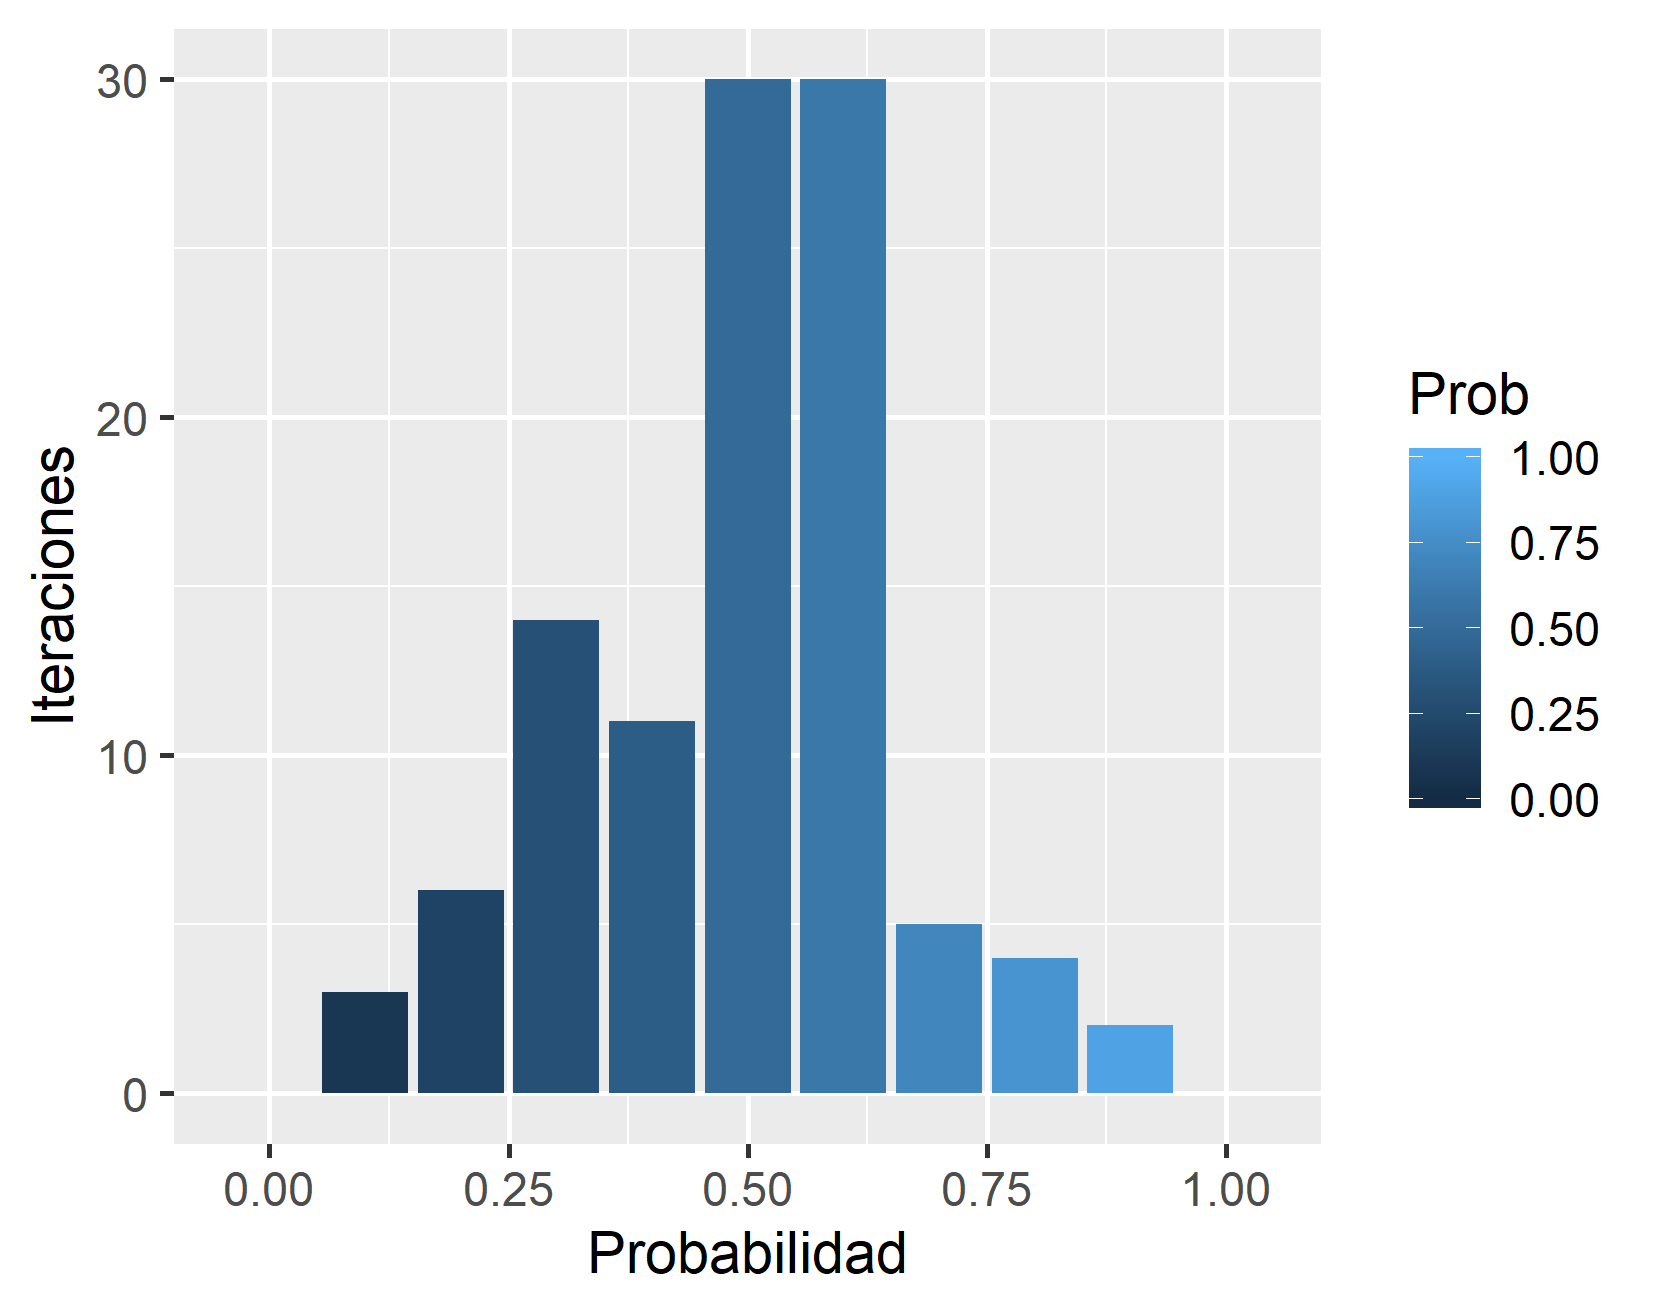
\includegraphics[width=80mm]{GraficaP2.png}
\caption{Gr\'afica en relaci\'on de probabilidades e iteraciones.}
\label{fig:Grafica}
\end{figure}

Cuando la probabilidad abarca los 0.50 hasta 0.80, la supervivencia de las celdas sobrepasa el l\'imite de iteraciones establecido (100), por lo tanto, estas celdas no llegan a morir.
El inicio de esta matr\'iz \ref{fig:Matriz} se encuentra animado con ayuda de Giphy \cite{Giphy}, en la carpeta de la pr\'actica 2 del repositorio.

\begin{figure}[h!]
\centering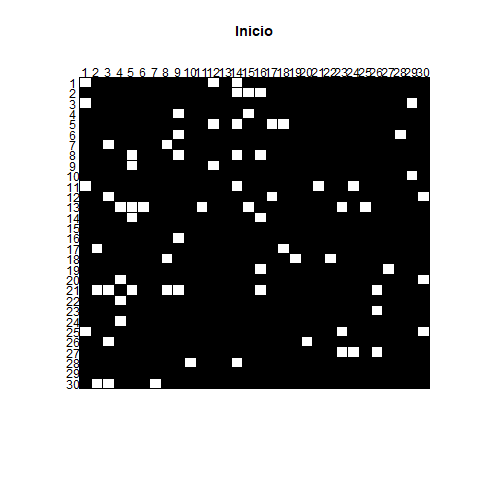
\includegraphics[width=100mm]{p2_Rep1_t0.png}
\caption{Matr\'iz inicial con probabilidad de 0.80}
\label{fig:Matriz}
\end{figure}

\section{Conclusi\'on}

De acuerdo a los datos obtenidos y mostrados en la gr\'afica:

\begin{enumerate}

\item{Las iteraciones aumentan cuando la probabilidad llega a ser un poco m\'as alta de la uniforme, con lo cual, le toma m\'as iteraciones para que estas se mueran.}

\item{En casos donde la probabilidad llega a ser de cero y uno, toman la menor de las iteraciones posibles siendo estas de cero.}

\end{enumerate}

\newpage

\bibliographystyle{plainnat}
\bibliography{Bibliografias}
\end{document}